\documentclass[11pt,a4paper]{article} 

\usepackage[dutch]{babel} %needs to specified for minutes package (else it will be in German)
\usepackage{a4wide}%For a wider spacing of the text (smaller left/right margin)
\usepackage{graphicx}
\usepackage{setspace}
\usepackage{minutes}

\pagestyle{plain}
\usepackage{todositemized}
%more memmorable commands to make the checked and crossed symbols





%%%%%%%%%%%%%%%%%%%%%%%%%%%%%%%%%%%%%%%%%%%%%%%%%%%%%%%%%%%%%%%%%%%%%%%%%%%%%%%
%
% Important: This template compiles without errors
% always check errors, also the yellow ones, even if you get a PDF
%
%%%%%%%%%%%%%%%%%%%%%%%%%%%%%%%%%%%%%%%%%%%%%%%%%%%%%%%%%%%%%%%%%%%%%%%%%%%%%%%%





\newpage



\usepackage[dutch]{babel} %needs to specified for minutes package (else it will be in German)
\usepackage{a4wide}%For a wider spacing of the text (smaller left/right margin)

\usepackage{setspace}
\usepackage{minutes}

\pagestyle{plain}
\usepackage{todositemized}
%more memmorable commands to make the checked and crossed symbols





%%%%%%%%%%%%%%%%%%%%%%%%%%%%%%%%%%%%%%%%%%%%%%%%%%%%%%%%%%%%%%%%%%%%%%%%%%%%%%%
%
% Important: This template compiles without errors
% always check errors, also the yellow ones, even if you get a PDF
%
%%%%%%%%%%%%%%%%%%%%%%%%%%%%%%%%%%%%%%%%%%%%%%%%%%%%%%%%%%%%%%%%%%%%%%%%%%%%%%%%



\begin{document}

\begin{Minutes}{Notulen Poject Natuurkunde, groepje 24}


%Add relevant date, time and location here
\minutesdate{04-06-2023} %Write the date of when you finish the minutes
\starttime{11:00}
\endtime{}
\location{}

%Add relevant names here
\participant{Tom, Talha, Madelief, Noah} 
\minutetaker{Madelief}

% \moderation{Niemand} 
%In case people are not present


\maketitle



\newpage


\section{Mededelingen} 
Vandaag hebben Talha en Madelief vooral verder gewerkt aan de experimenten met de silly putty en de opstelling. Tom en Noah hebben aan de code gewerkt voor het bepalen van de snelheid van de putty voor en na de vervorming. We zijn van 11 tot 5 bezig geweest vandaag.

\section{Experiment}
We hebben de opstelling weer gebruikt zoals staat genoteerd in de notulen van 3 juni. Vandaag hebben we ongeveer 10 tests gedaan met silly putty door het van verschillende hoogtes te laten vallen.

Ook was er een nieuw idee bedacht om de adhesie tegen te gaan. We willen namelijk maizena op de silly putty doen zodat het niet meer tegen het glas aanplakt. Blijkbaar verandert het de eigenschappen van de silly putty niet, al lijkt het mij wel dat de impact minder elastisch wordt.

\section{Wat moeten we nu doen/bespreken?}
We gaan de test met en zonder maizena gewoon uitvoeren en vergelijken, maar het is wellicht toch handig om nog wat te bespreken/onderzoeken over de impact van maizena op de eigenschappen van silly putty.



\section{Figuren}
\begin{figure}[h]
    \centering
    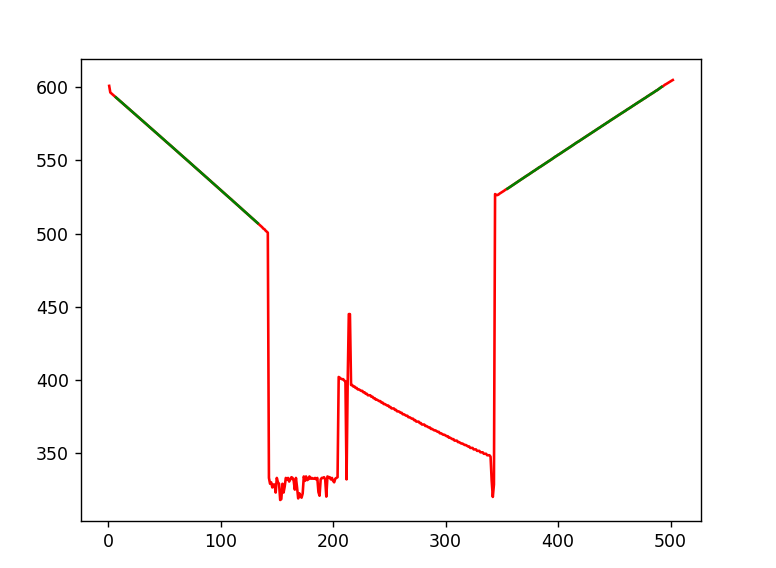
\includegraphics[width=0.5\linewidth]{Snelheidbepalen.png}
    \caption{Voorbeeld van de data verzameld voor het bepalen van de snelheid van de putty voor en na de rebound}
    \label{fig:enter-label}
\end{figure}

\listoftasks


\end{Minutes}
\end{document}


\section{Oude actiepunten}
Zijn er niet.

\section{Wat moeten we nu doen/bespreken?}

\subsection{Wie wil en kan wat?}

\task{talha}{checklist}

\subsection{Communicatie}


\subsection{Beschikbaarheid}


\section{Checklist uit de Powerpoint}



\section{Overige punten}
We wachten even morgen af, als we met Antoine spreken.

\section{Nieuwe actiepunten}
\listoftasks
\section{Volgende vergadering}
De volgende bijeenkomst is morgen met de begeleider, bij het fancy koffiezet apparaat bij D.

\section{Afsluiting vergadering}
De vergadering is om 12:49 gesloten.


\end{Minutes}
\end{document}